\section{Flow\-Shop\-Op\-Crossover\-Quad Class Reference}
\label{classFlowShopOpCrossoverQuad}\index{FlowShopOpCrossoverQuad@{FlowShopOpCrossoverQuad}}
Quadratic crossover operator for flow-shop (modify the both genotypes).  


{\tt \#include $<$Flow\-Shop\-Op\-Crossover\-Quad.h$>$}

Inheritance diagram for Flow\-Shop\-Op\-Crossover\-Quad::\begin{figure}[H]
\begin{center}
\leavevmode
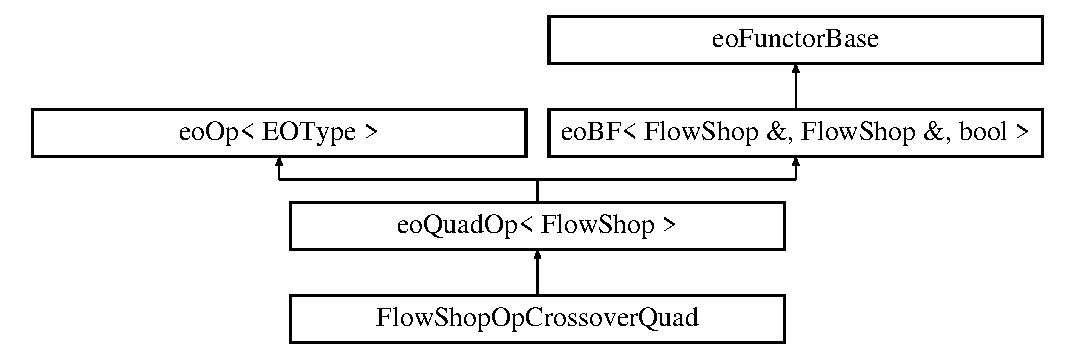
\includegraphics[height=4cm]{classFlowShopOpCrossoverQuad}
\end{center}
\end{figure}
\subsection*{Public Member Functions}
\begin{CompactItemize}
\item 
std::string \bf{class\-Name} () const \label{classFlowShopOpCrossoverQuad_60ac69b87970b7000980f65aa6ead44a}

\begin{CompactList}\small\item\em the class name (used to display statistics) \item\end{CompactList}\item 
bool \bf{operator()} (\bf{Flow\-Shop} \&\_\-flowshop1, \bf{Flow\-Shop} \&\_\-flowshop2)
\begin{CompactList}\small\item\em eo\-Quad crossover - \_\-flowshop1 and \_\-flowshop2 are the (future) offspring, i.e. \item\end{CompactList}\end{CompactItemize}
\subsection*{Private Member Functions}
\begin{CompactItemize}
\item 
\bf{Flow\-Shop} \bf{generate\-Offspring} (const \bf{Flow\-Shop} \&\_\-parent1, const \bf{Flow\-Shop} \&\_\-parent2, unsigned int \_\-point1, unsigned int \_\-point2)
\begin{CompactList}\small\item\em generation of an offspring by a 2 points crossover \item\end{CompactList}\end{CompactItemize}


\subsection{Detailed Description}
Quadratic crossover operator for flow-shop (modify the both genotypes). 



Definition at line 47 of file Flow\-Shop\-Op\-Crossover\-Quad.h.

\subsection{Member Function Documentation}
\index{FlowShopOpCrossoverQuad@{Flow\-Shop\-Op\-Crossover\-Quad}!operator()@{operator()}}
\index{operator()@{operator()}!FlowShopOpCrossoverQuad@{Flow\-Shop\-Op\-Crossover\-Quad}}
\subsubsection{\setlength{\rightskip}{0pt plus 5cm}bool Flow\-Shop\-Op\-Crossover\-Quad::operator() (\bf{Flow\-Shop} \& {\em \_\-flowshop1}, \bf{Flow\-Shop} \& {\em \_\-flowshop2})\hspace{0.3cm}{\tt  [virtual]}}\label{classFlowShopOpCrossoverQuad_92f70807bea24d3c233af580e2c55e3a}


eo\-Quad crossover - \_\-flowshop1 and \_\-flowshop2 are the (future) offspring, i.e. 

\_\-copies\_\- of the parents \begin{Desc}
\item[Parameters:]
\begin{description}
\item[{\em \_\-flowshop1}]the first parent \item[{\em \_\-flowshop2}]the second parent \end{description}
\end{Desc}


Implements \bf{eo\-BF$<$ Flow\-Shop \&, Flow\-Shop \&, bool $>$}.

Definition at line 47 of file Flow\-Shop\-Op\-Crossover\-Quad.cpp.

References generate\-Offspring(), eo\-Rng::random(), and moeo\-Vector$<$ MOEOObjective\-Vector, MOEOFitness, MOEODiversity, Gene\-Type $>$::value().\index{FlowShopOpCrossoverQuad@{Flow\-Shop\-Op\-Crossover\-Quad}!generateOffspring@{generateOffspring}}
\index{generateOffspring@{generateOffspring}!FlowShopOpCrossoverQuad@{Flow\-Shop\-Op\-Crossover\-Quad}}
\subsubsection{\setlength{\rightskip}{0pt plus 5cm}\bf{Flow\-Shop} Flow\-Shop\-Op\-Crossover\-Quad::generate\-Offspring (const \bf{Flow\-Shop} \& {\em \_\-parent1}, const \bf{Flow\-Shop} \& {\em \_\-parent2}, unsigned int {\em \_\-point1}, unsigned int {\em \_\-point2})\hspace{0.3cm}{\tt  [private]}}\label{classFlowShopOpCrossoverQuad_cbc2f344a0a29861900f4846597564c3}


generation of an offspring by a 2 points crossover 

\begin{Desc}
\item[Parameters:]
\begin{description}
\item[{\em \_\-parent1}]the first parent \item[{\em \_\-parent2}]the second parent \item[{\em \_\-point1}]the first point \item[{\em \_\-point2}]the second point \end{description}
\end{Desc}


Definition at line 80 of file Flow\-Shop\-Op\-Crossover\-Quad.cpp.

Referenced by operator()().

The documentation for this class was generated from the following files:\begin{CompactItemize}
\item 
Flow\-Shop\-Op\-Crossover\-Quad.h\item 
Flow\-Shop\-Op\-Crossover\-Quad.cpp\end{CompactItemize}
